\section{X-CANIDS Replication and Comparison with IWSHAP}
\label{sec:iwshap-comparison}

To assess whether the architectural trade-off persists in another feature space and to enable an external comparison, a replication used the two public X-CANIDS scenarios adopted by IWSHAP~\cite{Scherer2024IWSHAP}. The public code was pinned at commit \texttt{fb0d3093c12421d08ab3fb595d20c29ba2442e65}. Each scenario contains 20,000 records and 688 predictors. The controlled 60/20/20 split grouped identical complete vectors so that duplicates could not cross training, validation, and test. Suspension yielded 12,081/3,892/4,027 records and fabrication yielded 11,944/3,994/4,062, respectively.

Running the original code with pandas 2.2.2, NumPy 1.26.4, SHAP 0.45.1, XGBoost 2.0.3, and scikit-learn 1.5.0 reproduced, for fabrication, positive-class F1 0.787387 and the four-feature subset in the historical log. For suspension, it obtained positive F1 0.635693 with two features, unlike the 0.918619 and 16 features recorded in the June log. That log reports neither a hash nor a row count, so it is not assumed to correspond to the 20,000-row file. Moreover, the original program encodes categories before the 80/20 split and reuses the same 20\% during selection and for the reported result; these values are reproduction evidence, not held-out testing.

A new campaign compared G-FShield and Monolith~2 with the same ReliefF--VND--IWSSR sequence. It used 30 paired seeds per scenario, a 1,080-s selection window within the 1,200-s limit, at most 50 accepted improvements, three distributed consumers, and a common ceiling of six CPUs and 12~GiB. All 120 runs finished valid. SHA-256 was recalculated for all 120 manifests and the 1,500 files they enumerate, with no mismatch. Table~\ref{tab:iwshap-architecture} shows that the replication confirmed the concurrent mechanism and higher IWSSR throughput, but also confirmed its resource cost and lack of latency advantage.

\begin{landscape}
\begin{table}[p]
\centering
\scriptsize
\caption{X-CANIDS architectural replication: medians of 30 seeds per architecture and scenario.}
\label{tab:iwshap-architecture}
\resizebox{.98\linewidth}{!}{%
\begin{tabular}{llrrrrrr}
\toprule
\textbf{Scenario} & \textbf{Architecture} & \textbf{Test macro-F1} & \textbf{Time to baseline (s)} & \textbf{IWSSR/s} & \textbf{CPU-s} & \textbf{Peak RAM (MiB)} & \textbf{Overlap} \\
\midrule
Suspension & G-FShield & 0.790717 & 114.463 & 8.580 & 3,853.1 & 3,370.3 & 99.657\% \\
Suspension & Monolith & 0.787396 & 92.071 & 3.698 & 1,100.7 & 770.1 & 0\% \\
Fabrication & G-FShield & 0.902245 & 101.047 & 8.302 & 3,858.4 & 3,169.8 & 99.664\% \\
Fabrication & Monolith & 0.900280 & 90.091 & 3.678 & 1,096.9 & 774.6 & 0\% \\
\bottomrule
\end{tabular}}
\end{table}
\end{landscape}

Final macro-F1 did not differ after Holm correction: for suspension, the paired median difference was $+0.000665$ (95\% bootstrap CI from 0 to $+0.005313$; $p_{Holm}=0.438598$); for fabrication, it was zero ($p_{Holm}=1$). In contrast, anytime AUC favored the monolith in all 30 pairs of both scenarios ($p_{Holm}\approx0.000030$). Time to the all-feature validation baseline was also shorter for the monolith, but is only descriptive because that threshold, although computed before the campaign, was not embedded in the frozen manifest. The distributed arm evaluated IWSSR candidates approximately 2.3 times faster and overlapped local search with construction for more than 99.65\% of the window, at the cost of about 3.5 times as many CPU-seconds and approximately four times the peak RAM.

To compare selectors without confounding classifier and split, every frozen subset was retrained on training data only and evaluated with the same XGBoost; validation supported analysis and the held-out test was queried once. Table~\ref{tab:iwshap-xgboost} separates this controlled comparison from published numbers and from the reproduction that reuses the selection set.

\begin{landscape}
\begin{table}[p]
\centering
\scriptsize
\caption{Subsets evaluated by the same XGBoost on the same held-out test. G-FShield and monolith values are medians of 30 seeds; fixed comparators have one run.}
\label{tab:iwshap-xgboost}
\resizebox{.98\linewidth}{!}{%
\begin{tabular}{llrrrrrr}
\toprule
\textbf{Scenario} & \textbf{Method} & \textbf{$n$} & \textbf{Features} & \textbf{Reduction} & \textbf{Macro-F1} & \textbf{Positive F1} & \textbf{Positive precision/recall} \\
\midrule
Suspension & All features & 1 & 688 & 0\% & 0.734966 & 0.532915 & 0.517241 / 0.549569 \\
Suspension & Historical IWSHAP subset & 1 & 16 & 97.67\% & 0.830048 & 0.699894 & 0.688935 / 0.711207 \\
Suspension & G-FShield & 30 & 20.5 & 97.02\% & 0.723518 & 0.511074 & 0.511256 / 0.510776 \\
Suspension & Paired monolith & 30 & 21 & 96.95\% & 0.723544 & 0.510315 & 0.513282 / 0.507543 \\
Fabrication & All features & 1 & 688 & 0\% & 0.882397 & 0.795019 & 0.750452 / 0.845214 \\
Fabrication & Historical IWSHAP subset & 1 & 4 & 99.42\% & 0.882423 & 0.799667 & 0.675562 / 0.979633 \\
Fabrication & G-FShield & 30 & 17 & 97.53\% & 0.887680 & 0.803178 & 0.787196 / 0.820774 \\
Fabrication & Paired monolith & 30 & 17 & 97.53\% & 0.889053 & 0.805639 & 0.788703 / 0.823829 \\
\bottomrule
\end{tabular}}
\end{table}
\end{landscape}

For suspension, none of the 30 G-FShield runs exceeded the historical IWSHAP subset in macro-F1 or positive F1. For fabrication, 26 of 30 exceeded it in macro-F1 and 16 of 30 in positive F1. The highest observed value was macro-F1 0.900958 for G-FShield seed 20260916, with 19 features and positive F1 0.826347. However, the distributed median selected 17 features rather than IWSHAP's four and traded recall for precision: 0.820774/0.787196 versus 0.979633/0.675562. Because the IWSHAP subset is a fixed comparator, these counts and differences are descriptive rather than paired superiority tests. The external conclusion is scenario-dependent: G-FShield has a descriptive F1 advantage for fabrication, not for suspension, and does not simultaneously dominate quality, reduction, and recall.

\begin{landscape}
\begin{figure}[p]
  \centering
  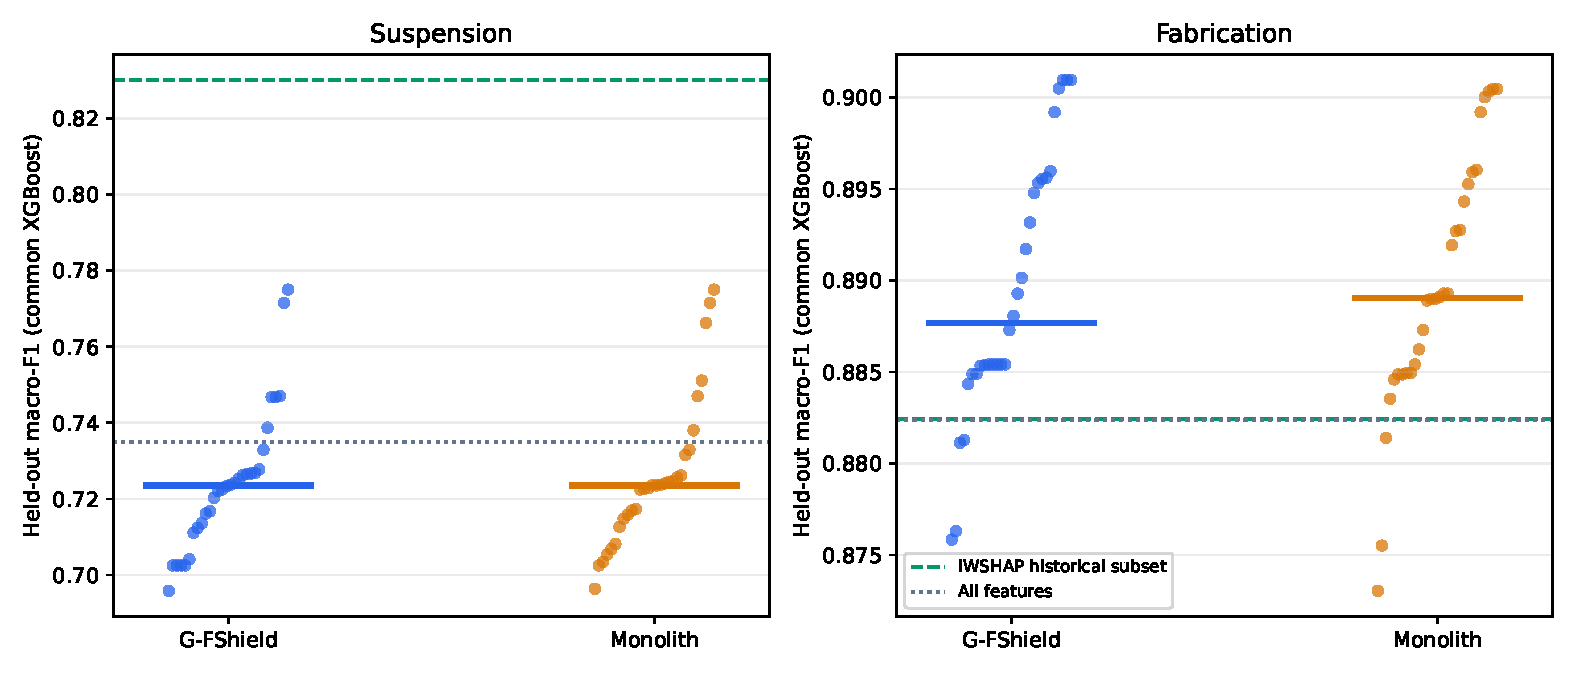
\includegraphics[width=.96\linewidth,height=.80\textheight,keepaspectratio]{fig/gfshield/iwshap-xgboost-common-comparison.pdf}
  \caption{Macro-F1 of frozen subsets under the common XGBoost protocol. Horizontal lines show the fixed all-feature and historical-IWSHAP-feature comparators.}
  \label{fig:iwshap-xgboost}
\end{figure}
\end{landscape}
